\chapter{算法与结果}
\label{cha:result}

\section{exRNA数据的收集与预处理}
\label{sec:first}

\subsection{exRNA数据收集}
我们收集整理了实验室自产的一套和两套发表的exRNA-seq数据,为了后续方便,我们称细胞外游离的RNA测序数据为cfRNA-seq,外泌体的RNA测序数据为exoRNA-seq. 同时我们用L(long)和S(small)区分长RNA和小RNA测序数据。一共四种主要的数据类型: S-cfRNA-seq, S-exoRNA-seq, L-cfRNA-seq, L-exoRNAs-eq. 我们收集的数据的具体信息如下:S-exoRNA-seq 数据来自于 GEO 数据库中收录的 GSE71008 (\cite{yuan2016plasma}),包含健康供体(healthy donor, HD)的 50 个,结直肠癌100 个(colorectal cancer, CRC)样本,前列腺癌(prostate adenocarcinoma, PRAD)36 个。  S-cfRNA-seq ,我们整理了实验室内部产生的数据GSE123972 (\cite{tan2019noncoding}) 以及GSE113994(\cite{max2018human}),GSE53080(\cite{giraldez2018comprehensive}) 和 GSE94582(\cite{akat2014comparative});GSE123973 有可用的肝癌(hepatocellular carcinoma, HCC) 样本30例,其中包括早期肝癌(HCC stageA)16个,健康供体(HD)的 13 个样本。 GSE113994包含53健康供体,GSE53080包含17健康供体,GSE94582包含20健康供体。对于 L-exoRNA-seq 数据,我们收集exoRBase数据库(\cite{li2017exorbase})中的数据,其源于多个实验室的合作,包括肝癌样本14个,结肠癌样本12个,胰腺癌样本14个和健康供体32个。
数据总结如~\ref{tab:exRNAsumtable}所示

\begin{table}[htb]
  \centering
  \begin{minipage}[t]{0.9\linewidth} % 如果想在表格中使用脚注,minipage是个不错的办法
  \caption[exRNA数据收集总结]{exRNA数据收集总结}%{模板文件。如果表格的标题很长,那么在表格索引中就会很不美}
  \label{tab:exRNAsumtable}
  %210pt in total
    \begin{tabularx}{\linewidth}{p{70pt}|p{80pt}|p{110pt}|p{70pt}}
      \toprule[1.5pt]
      {\heiti Data type} & {\heiti Sources}  & {\heiti Sample class} & {\heiti Sample size}\\\midrule[1pt]   
      S-exoRNA-seq & GSE71008 & \textbf{CRC}, PRAD, HD & 186\\
      S-cfRNA-seq & GSE123972 & \textbf{HCC}, HD & 43\\
      S-cfRNA-seq & GSE113994 & HD & 53\\
      S-cfRNA-seq & GSE53080 & HD & 17\\
      S-cfRNA-seq & GSE94582 & HD & 20\\
      L-exoRNA-seq & exoRBase & \textbf{HCC}, CRC, PRAD, HD & 20\\
      % (\cite{yuan2016plasma}) (\cite{tan2019noncoding}) (\cite{max2018human}) (\cite{giraldez2018comprehensive}) (\cite{akat2014comparative}) (\cite{li2017exorbase})
      \bottomrule[1.5pt]
    \end{tabularx}
  \end{minipage}
\end{table}

\paragraph{exRNA测序数据的处理}
针对exRNA数据微量性的特点,我们转门设计了小RNA测序数据的顺序比对方法,确定了其比对的先后顺序。完整的流程如~\ref{fig:reads_processing}所示。包括数据清洗,质量控制,顺序比对(针对小RNA)或序列比对,以及构建

\begin{figure}[H] % use float package if you want it here
    \centering
    \includegraphics[width = 0.8\textwidth]{reads_processing}
    \caption{reads处理流程图}
    \label{fig:reads_processing}
\end{figure}

\subsection{长exRNA测序数据的处理}

~\ref{fig:exorbase_basic} ,数据来源为exoRBase。 (A) 不同RNA映射比例的饼图; (B) 不同RNA的长度分布的三维条形图;
(C) 不同RNA的映射比例的箱线图 (D) 每个样本各种RNA映射比例的叠加条形图。
\begin{figure}[H] % use float package if you want it here
    \centering
    \includegraphics[width = 0.8\textwidth]{exorbase_basic}
    \caption{L-exoRNA-seq数据mapping基本情况统计。}
    \label{fig:exorbase_basic}
\end{figure}





\subsection{小exRNA测序数据的处理}

~\ref{fig:lulab_basic},数据来源为GSE123973。 (A) 不同RNA映射比例的饼; (B) 不同RNA的长度分布的三维条形图;
(C) 不同RNA的映射比例的箱线图 (D) 每个样本各种RNA映射比例的叠加条形图。
\begin{figure}[H] % use float package if you want it here
    \centering
    \includegraphics[width = 0.8\textwidth]{lulab_basic}
    \caption{S-cfRNA-seq数据mapping基本情况统计}
    \label{fig:lulab_basic}
\end{figure}

\section{表达矩阵的构建}
\label{sec:second}

图~\ref{fig:length_distribution}使用三维条状图和折线图展示了S-cfRNA-seq数据的各种类型RNA的长度分布。
\begin{figure}[h]
\centering%
\begin{subfigure}{0.4\textwidth}
\includegraphics[height=6cm]{3d_bar}
\caption{RNA长度分布的三维条形图展示}
\end{subfigure}%
\hspace{4em}%
\begin{subfigure}{0.4\textwidth}
\includegraphics[height=7cm]{length_distribution}
\caption{RNA长度分布的折线图图展示}
\end{subfigure}
\caption{RNA长度分布}
\label{fig:length_distribution}
\end{figure}

\subsection{结构域检测算法}

零阶段负二项分布(Zero Truncated Negative Binomial, ZTNB)模型如公式~\ref{equ:ZTNB}所示,其中r为实验指定的失败次数,也称分散系数,x为此时的成功次数,p为每次实验成功概率。$\Gamma$为伽马函数,如公式~\ref{equ:gamma}所示。
\begin{equation}\label{equ:ZTNB}
    p ( x ) = \left[ \Gamma ( x + r ) p^r ( 1 - p )^x \right] \left[ \Gamma ( n ) x ! \left( 1 - p ^r \right) \right]  
\end{equation}

\begin{equation}\label{equ:gamma}
    \Gamma ( x ) = \int _ { 0 } ^ { + \infty } t ^ { x - 1 } e ^ { - t } \mathrm { d } t
\end{equation}


图~\ref{fig:domain_example}
\begin{figure}[h]
    \centering%
    \begin{subfigure}{0.4\textwidth}
      \includegraphics[height=4.5cm]{peak_calling}
      \caption{结构域检测算法检测到的片段}
    \end{subfigure}%
    \hspace{4em}%
    \begin{subfigure}{0.4\textwidth}
      \includegraphics[height=4cm]{domain_example}
      \caption{结构域片段在exRNA和组织RNA数据中的比较}
    \end{subfigure}
    \caption{结构域检测算法检测到的片段举例}
    \label{fig:domain_example}
  \end{figure}


\subsection{结构域检测分析}


图~\ref{fig:ic_rbp}
\begin{figure}[h]
\centering%
\begin{subfigure}{0.3\textwidth}
\includegraphics[height=4cm]{icshape}
\caption{使用icSHAPE展示不同位置片段的结构特性}
\end{subfigure}%
\hspace{4em}%
\begin{subfigure}{0.4\textwidth}
\includegraphics[height=4cm]{rbp}
\caption{使用RBP binding数据展示不同位置片段与RBP结合的潜在可能性}
\end{subfigure}
\caption{结构域片段结构域RBP结合性分析}
\label{fig:ic_rbp}
\end{figure}


图~\ref{fig:domain_size}展示了XXXXXXXXXXXXXXX
\begin{figure}[h]
  \centering%
  \begin{subfigure}{0.4\textwidth}
    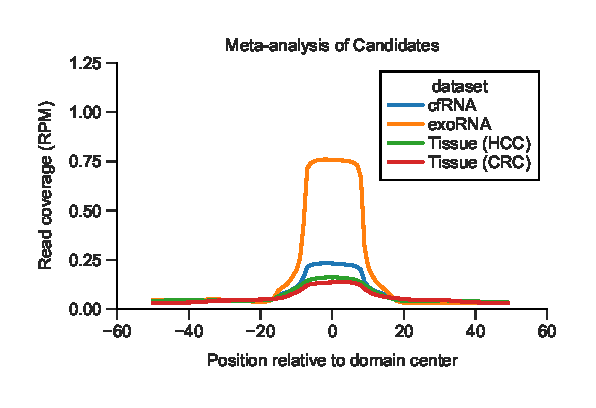
\includegraphics[height=5cm]{aggregation_plot}
    \caption{结构域分布}
  \end{subfigure}%
  \hspace{4em}%
  \begin{subfigure}{0.4\textwidth}
    \includegraphics[height=5cm]{domain_size}
    \caption{结构域大小分布}
  \end{subfigure}
  \caption{不同exRNA和组织数据结构域分布和大小分布}
  \label{fig:hcc_crc_auc_sum}
\end{figure}



图~\ref{fig:div_abu}
\begin{figure}[h]
  \centering%
  \begin{subfigure}{0.4\textwidth}
    \includegraphics[height=4cm]{diversity_abundance_cfRNA}
    \caption{S-cfRNA-seq结构域和miRNA特征的丰度与多样性}
  \end{subfigure}%
  \hspace{4em}%
  \begin{subfigure}{0.4\textwidth}
    \includegraphics[height=4cm]{diversity_abundance_scirep}
    \caption{S-exoRNA-seq结构域和miRNA特征的丰度与多样性}
  \end{subfigure}
  \caption{小exRNA-seq结构域和miRNA特征的丰度与多样性}
  \label{fig:div_abu}
\end{figure}






图~\ref{fig:diff_pie}
\begin{figure}[h]
  \centering%
  \begin{subfigure}{0.4\textwidth}
    \includegraphics[height=4cm]{piecharts_cfRNA}
    \caption{S-cfRNA-seq差异表达RNA比例}
  \end{subfigure}%
  \hspace{4em}%
  \begin{subfigure}{0.4\textwidth}
    \includegraphics[height=4cm]{piecharts_scirep}
    \caption{S-exoRNA-seq差异表达RNA比例}
  \end{subfigure}
  \caption{小exRNA-seq差异表达RNA比例}
  \label{fig:diff_pie}
\end{figure}

\section{表达矩阵的处理}
\label{sec:third}


\begin{figure}[H] % use float package if you want it here
    \centering
    \includegraphics[width = 0.7\textwidth]{matrix_processing}
    \caption{表达矩阵处理流程图}
    \label{fig:mx_process_pipe}
\end{figure}

%\subsection{过滤与归责处理}

\subsection{测序深度归一化}

~\ref{fig:rle}
\begin{figure}[H] % use float package if you want it here
    \centering
    \includegraphics[width = 0.8\textwidth]{RLE}
    \caption{样本库大小归一化效果}
    \label{fig:rle}
\end{figure}

\subsection{去除批次效应}

~\ref{fig:batch_correction}
\begin{figure}[H] % use float package if you want it here
    \centering
    \includegraphics[width = 0.65\textwidth]{batch_correction}
    \caption{去除批次效应效果}
    \label{fig:batch_correction}
\end{figure}

\subsection{评估表达矩阵处理效果}



非监督聚类准确性(unsupervised clustering accuracy, UCA)(\cite{lopez2018deep}),由一篇单细胞领域研究中首次适用,用于衡量聚类的效果,作为PCA和t-SNE等降维可视化分析的量化评估,可以使我们预先判断当前处理效果下数据的大致分类效果。
UCA首先只用K-means(\cite{jain1988algorithms})或者KNN(\cite{cover1967nearest})作为聚类的方法,由于是非监督聚类,还需要使用线性分配的算法如匈牙利算法(\cite{linearassign})将聚类标签与真实标签进行匹配。此时该问题可以看做一个有标签的分类问题,计算出分类的准确率即为非监督聚类准确性。
对于多种不同的聚类度量指标,我们发现UCA和有监督的分类度量指标AUC具有最强的相关性,因此采用非监督聚类准确性指标作为矩阵处理效果的度量之一。

为了更好地衡量批次效应的严重性以及批次效应去除效果,我们参考了过去的指标如对齐分数(alignment score)(\cite{butler2018integrating}),和kBET(\cite{buttner2017assessment})两个研究。对齐分数虽然计算简单,但是只适用于二分类标签,kBET使用时会遇到受到随机效应影响而导致极端值附近的结果不够稳定的情况。
为此我们提出了m-K最近邻 (m-K-nearest neighbor, mKNN)指标, 公式如式~(\ref{eq:mknn})所示,其中 $\bar x_b, k, N_b, N, B$ 分别表示:批次为b的样本周围同类批次的样本平均个数,自主定义的最近邻取样数,批次为b的样本总数,所有样本的总数以及批次的种类数。利用mKNN指标,我们可以逐批次逐样本地衡量其批次效应的严重性,
批次效应越严重,则分子中的$\bar x_b$越大,相应的整个指标越大。为了更好地表示“去除批次效应的效果”,我们使用1-mKNN作为去除批次效应效果的指标。
\begin{equation}
\label{eq:mknn}
\frac { 1 } { B } \sum _ { b = 1 } ^ { B } \frac { \overline { x } _ { b } - k N _ { b } / ( N - 1 ) } { \min \left( k , N _ { b } \right) - k N _ { b } / ( N - 1 ) }
\end{equation}

UCA和mKNN指标均为$0\sim 1$,数值越大代表聚类效果越好以及批次效应的影响越小。因此我们统一地考虑两个指标,将矩阵处理方法的组合(即测序深度归一化以及去除批次效应方法的组合)加以统一的评估。~\ref{fig:matrix_processing_metric}中每一个点表示一种矩阵
处理方法的组合。越靠近右上角的指标代表矩阵处理效果越好。如图所示,我们可以选择RLE作为测序深度归一化加上Limma作为去除批次效应的方法组合。对于该方法组合,我们还是用了PCA对矩阵处理前后的数据进行了可视化,PCA可以用于降维,选择方差贡献最大的两个主成分表示到二维平面上,点的颜色表示批次,性状表示类别信息。
不管是视觉上观察可以看到不同批次的点更好的混在了一起,还是从两个指标的变化($\text{UCA}:0.519 \rightarrow 0.692; \text{mKNN}:0.055 \rightarrow 0.792$)上,均可以得出矩阵处理方法较好地完成了测序深度归一化以及批次效应去除的任务的结论。

\begin{figure}[H] % use float package if you want it here
    \centering
    \includegraphics[width = 0.8\textwidth]{matrix_processing_metric}
    \caption{综合使用UCA和mKNN评估矩阵处理效果}
    \label{fig:matrix_processing_metric}
\end{figure}

\section{特征选择和模型评估}
\label{sec:fourth}
由矩阵处理流程处理好的表达矩阵消除了部分技术性差异(technical variance)导致的样本库大小不一致和批次效应问题。
我们可以对处理过的表达矩阵应用一些统计学习模型,设计一套特征选择流程,选取对于癌症和正常样本分类效果好的,稳定的,具有生物学意义的特征,作为癌症检测的潜在的生物标志物。

\subsection{差异表达分析}
差异表达分析可以使用统计模型逐基因地寻找在癌症和正常人之间差异表达的特征。因为也可以作为
特征选择的基本方法之一。


% 讨论deseq的基本原理,注意表达要修改
我们使用DESeq2包进行差异表达分析,值得注意的是DESeq2专门要求输入的矩阵必须是基因计数矩阵,也就是未经标准化和归一化的表达矩阵(un-normalized counts)(\cite{love2014moderated}). 因为这样的矩阵具有最多的信息和准确性,DESeq2在内部会自动完成归一化的工作。

DESeq2为了比较两组样本之间的计数差异建立了一个模型。该模型包含以下参数:(1)归一化参数,至少可以归一化库大小的差异; (2)方差参数,也被成为分散系数(dispersion); (3)表示组间差异的参数。DESeq2使用与原始DESeq相同的方法拟合(1)。拟合(2)分两步:首先找到使似然(likelihood)最大的参数值,即完成最大似然估计。查找所有的基因表达值,并将这些值向中间值移动,移动的量由贝叶斯模型给定:如果基因的信息较低,则值更多地移动到中间,如果基因的信息很大,则值移动很少。使用与(2)中使用的相同的技术拟合(3)。 (3)的值是最终需要得到的输出,找到一组组间差异高于某个数值的基因集合。这个阈值一般由错误发现率(False Discovery Rate, FDR)规定,一般取从小到大排最小的十个FDR基因作为差异表达基因。

对于差异表达基因的选取,这里我们使用一个改进的指标以替代FDR,该指标如~\ref{equ:demetric}所示,可以综合性考虑FDR和fold change,更加完善。

\begin{equation}\label{equ:demetric}
  \pi = \| \log _ { 2 } F C | \cdot \left( - \log _ { 10 } \mathrm { FDR } \right)
\end{equation}


%compare counts between two groups. We build a model for the observed counts. This model has some parameters: (1) a normalization parameter, for differences in library size at least, or it can be extended by other software; (2) a variance parameter, called dispersion; (3) parameters representing the group differences. Fit (1) using the same method from the original DESeq. Fit (2) in two steps: first find the value of the parameter that makes the  likelihood largest, which iscalled maximum likelihood estimation. Look at all the values from all of the genes and move these values towards a middle value. Bayes theorem guides the amount of movement for each gene: if the information for the gene is low, the value is moved more to the middle, if the information for the gene is high, the value is moved very little. Fit (3) using the same technique as used for (2). The values for (3) are a useful final product, as are sets of genes where the group differences are likely to be above a threshold (zero or otherwise). These sets are defined by their false discovery rate.

%TODO 展示基本的DE结果并简单讨论
使用DESeq2对原始的基因计数矩阵进行分析,可以得到如~\ref{fig:lulab_de}和~\ref{fig:scirep_de}的结果。


对于~\ref{fig:lulab_de},我们使用S-cfRNA-seq数据,癌症类型分别为肝癌和早期肝癌。将其分别与正常样本比较,可以分别找出可以区分正常样本与肝癌以及正常样本与早期肝癌的差异基因。
(A) 表示每个基因的对数fold change和对数调整后p值的火山图,图中红色的点为差异表达的基因,越靠近右上和左上的基因其差异表达越明显; (B) 前十个差异表达基因的
fold change, 表达值以及对数调整后p值; (C) 挑选出的差异表达基因的热图以显示其对于癌症和正常样本的分类效果。
的分类效果。
\begin{figure}[H] % use float package if you want it here
    \centering
    \includegraphics[width = 0.8\textwidth]{lulab_de}
    \caption{S-cfRNA-seq数据的差异表达分析}
    \label{fig:lulab_de}
\end{figure}

对于~\ref{fig:scirep_de},我们使用S-exoRNA-seq数据,癌症类型分别为结肠癌和早期结肠癌。图的具体信息与~\ref{fig:lulab_de}表示的类似。
\begin{figure}[H] % use float package if you want it here
    \centering
    \includegraphics[width = 0.8\textwidth]{scirep_de}
    \caption{S-exoRNA-seq数据的差异表达分析}
    \label{fig:scirep_de}
\end{figure}

差异表达分析的模型一般会独立考虑每个特征(即基因)的贡献,并不能结合性地讨论特征对
分类的共同贡献,因此有局限性。接下来我们将会使用一些经典的机器学习模型来更好地组合
不同的特征,以选出一组生物学上更有解释性和代表性的基因作为可能的生物标志物。同时考虑
到模型必须具有的泛化能力以及稳定性,我们还会针对性地设计一个特征选择的框架来更好的挑选特征。

\subsection{特征选择策略与机器学习模型}

\paragraph{特征选择框架}


%~\ref{fig:fs_frame}
%\begin{figure}[H] % use float package if you want it here
%    \centering
%    \includegraphics[width = 0.6\textwidth]{fs_frame}
%    \caption{特征选择框架}
 %   \label{fig:fs_frame}
%\end{figure}

特征选择算法~\ref{alg:fs_algorithm}

%feature selection算法

\begin{algorithm}
\caption{稳健的特征选择算法}\label{alg:fs_algorithm}
\begin{algorithmic}[1]
\STATE Scale each feature independently using robust normalization;
\FOR{feature\_num $k \in [1,10], 20, 30, 40, 50$}
\STATE Random select 90\% samples for 50 times;
\STATE Run a classifier (Random Forest, Logistic Regression or Linear SVM) to select features based on feature importance. 
	\FOR{each classifier $\in$ [Random Forest, Logistic Regression or Linear SVM]}
	\STATE Optimize classifier's hyper-parameters by 5-fold cross-validation;
	\ENDFOR
\STATE Select top k features that are recurrently selected across resampling runs;
\STATE Calculate AUC mean;
\ENDFOR
\STATE Rank processing method by AUC, select the best processing method;
\STATE Select union of features in different feature\_num setting. Refit by selecting $i \in [1,10]$ features and calculate feature importance.
\end{algorithmic}
\end{algorithm}




\paragraph{机器学习模型}
在特征选择框架中我们可以选择多种机器学习模型,包括逻辑斯谛回归(\cite{kleinbaum2002logistic}),支持向量机(\cite{scholkopf2001learning}),随机森林(\cite{liaw2002classification})等。
以逻辑斯谛回归为例,对于二分类问题,逻辑斯谛回归的决策模型如公式~\ref{equ:logistic}所示,其中$x$为表达矩阵,$\beta$为逻辑斯谛回归中线性模型的权重向量,$\beta_0$为偏置项。公式~\ref{equ:logistic}表示输入为$x$时模型判断样本标签为1的概率。若设患癌症样本的标签为1,则代表该样本为癌症患者的概率。
\begin{equation}\label{equ:logistic}
    P ( Y = 1 | X = x ) = \frac { \exp \left( \beta _ { 0 } + x ^ { T } \beta \right) } { 1 + \exp \left( \beta _ { 0 } + x ^ { T } \beta \right) }
\end{equation}

类似地可以得到多分类的逻辑斯谛回归如公式~\ref{equ:multilogistic}


\begin{subequations}\label{equ:multilogistic}
\begin{flalign}
    & P ( Y = k | X = x ) = \frac { \exp \left( \beta _ { k , 0 } + x ^ { T } \beta _ { k } \right) } { 1 + \sum _ { l = 1 } ^ { K - 1 } \exp \left( \beta _ { l , 0 } + x ^ { T } \beta _ { l } \right) } , \text { for } k = 1 , \ldots , K - 1\\ 
    & P ( Y = K | X = x ) = \frac { 1 } { 1 + \sum _ { l = 1 } ^ { K - 1 } \exp \left( \beta _ { l , 0 } + x ^ { T } \beta _ { l } \right) } , \text { for } k = K
\end{flalign}
\end{subequations}

\subsection{特征选择的分类效果和稳健性评估}

Kuncheva index公式如式~(\ref{eq:ki}),其中 $f_i, f_j$ 为两次挑选的特征,$d, N$ 分别为一次挑选的特征数和总特征数量。
\begin{equation}\label{eq:ki}
\mathrm { KI } \left( f _ { i } , f _ { j } \right) = \frac { \left| f _ { i } \cap f _ { j } \right| N - d ^ { 2 } }{ d N - d ^ { 2 } } = \frac { \left| f _ { i } \cap f _ { j } \right| - d ^ { 2 } / N } { d - d ^ { 2 } / N }
\end{equation}

若做K次采样,均采取不放回的策略时,可以获得平均KI的公式如式~(\ref{eq:aki}),即AKI。

\begin{equation}\label{eq:aki}
\mathrm { AKI } = \frac { 2 } { M ( M - 1 ) } \sum _ { i = 1 } ^ { M } \sum _ { j = 1 } ^ { M } \mathrm { KI } \left( f _ { i } , f _ { j } \right)
\end{equation}


\subsection{模型分类效果比较总结}

图~\ref{fig:feature_selection_compare}
\begin{figure}[h]
  \centering%
  \begin{subfigure}{0.4\textwidth}
    \includegraphics[height=4cm]{feature_selection_erro_hcc_fig4a}
    \caption{结肠癌数据特征选择方法总结}
  \end{subfigure}%
  \hspace{4em}%
  \begin{subfigure}{0.4\textwidth}
    \includegraphics[height=4cm]{feature_selection_erro_hcc_fig4b}
    \caption{肝癌数据特征选择方法总结}
  \end{subfigure}
  \caption{特征选择方法总结}
  \label{fig:feature_selection_compare}
\end{figure}

图~\ref{fig:hcc_crc_auc_sum}汇总了S-cfRNA-seq和S-exoRNA-seq两套数据的肝癌(HCC和结肠癌(CRC)两种疾病不同生物标志物作为特征的分类效果。
\begin{figure}[h]
  \centering%
  \begin{subfigure}{0.4\textwidth}
    \includegraphics[height=5cm]{hcc_auc_sum_revise_fig4b_5}
    \caption{肝癌各生物标志物AUC总结}
  \end{subfigure}%
  \hspace{4em}%
  \begin{subfigure}{0.4\textwidth}
    \includegraphics[height=5cm]{crc_auc_sum_revise_fig4b_5}
    \caption{结肠癌各生物标志物AUC总结}
  \end{subfigure}
  \caption{肝癌和结肠癌AUC总结}
  \label{fig:hcc_crc_auc_sum}
\end{figure}

~\ref{fig:compare_feature_num}
\begin{figure}[H] % use float package if you want it here
    \centering
    \includegraphics[width = 0.8\textwidth]{compare_feature_num}
    \caption{挑选不同数量feature时AUC的变化}
    \label{fig:compare_feature_num}
\end{figure}


\subsection{挑选出的候选生物标志物表现}
%ROC clustermap等

~\ref{fig:roc_curve}
\begin{figure}[H] % use float package if you want it here
    \centering
    \includegraphics[width = 0.4\textwidth]{roc_curve}
    \caption{早期肝癌分类的ROC曲线}
    \label{fig:roc_curve}
\end{figure}

~\ref{fig:candidate_sum}
\begin{figure}[H] % use float package if you want it here
    \centering
    \includegraphics[width = 1\textwidth]{candidate_sum}
    \caption{综合评估挑选的生物标志物}
    \label{fig:candidate_sum}
\end{figure}

\section{exSEEK软件介绍及使用}
\label{sec:fifth}





\subsection{软件基本功能模块与使用}

基于上述的工作我们开发了exSEEK软件,我们使用Snakemake软件包
(\cite{koster2012snakemake})对分析流程进行控制,
这是因为处理过程比较复杂,输出文件互相依赖,处理耗时长且
容易出现断点,使用Snakemake可以保证样本处理的管理有序。
exSEEK包含了三大模块,如图~\ref{fig:exseekmodule}所示,
Utilities和Preprocess模块包含了数据前处理,映射和构建表
达矩阵等功能,可用于L-exRNA-seq和S-exRNA-seq数据的映射
和表达矩阵构建。exSEEK模块为核心模块,可以完成差异表达,
矩阵处理以及特征挑选以及标志物评估等功能。exSEEK软件读取
一个可以由用户简洁地自定义的config.json文件用于设置各个
模块的相关参数,运行各个模块的具体步骤时均只需要一行命令
即可完成,方便各类用户使用。

\begin{figure}[h]
    \centering%
    \begin{subfigure}{0.4\textwidth}
      \includegraphics[height=3.5cm]{exSEEK_module}
      \caption{exSEEK软件模块示意图}
    \end{subfigure}%
    \hspace{4em}%
    \begin{subfigure}{0.4\textwidth}
      \includegraphics[height=3.5cm]{command}
      \caption{exSEEK软件使用命令}
    \end{subfigure}
    \caption{exSEEK软件模块及使用命令}
    \label{fig:exseekmodule}
  \end{figure}


\subsection{软件绘图模块及使用}




exSEEK软件还包含有高度可交互以及高度标准化的绘图模块
,如图~\ref{fig:jupyter}所示,我们使用jupyter$-$notebook
(\cite{kluyver2016jupyter})进行绘图模块的构建,
用户可以交互式地使用绘图模块完成高质量的结果可视化,只
需要选择相应的参数即可自动地产生类似本文配图的输出结果图。

\begin{figure}[H] % use float package if you want it here
    \centering
    \includegraphics[width = 0.8\textwidth]{jupyter}
    \caption{exSEEK绘图模块}
    \label{fig:jupyter}
\end{figure}

